By Section \ref{Numerical methods for computing the Casimir energy}, to compute the Casimir energy, we have to evaluate 
$\log\frac{\det\mathsf{V}_{\mathrm{i}k}}{\det\tilde{\mathsf{V}}_{\mathrm{i}k}} = \log\det(\mathsf{V}_{\mathrm{i}k}\tilde{\mathsf{V}}_{\mathrm{i}k}^{-1})$ 
with different values of $k$. In this section, an efficient inverse-free method will be introduced to compute this log determinant.

The log determinant of the matrix $\mathsf{V}_{\mathrm{i}k}\tilde{\mathsf{V}}_{\mathrm{i}k}^{-1}$ is equal to the sum of the logarithm of each eigenvalue of 
$\mathsf{V}_{\mathrm{i}k}\tilde{\mathsf{V}}_{\mathrm{i}k}^{-1}$. From Figure \ref{eigenvalues of VVtilde}, we can notice that most of the eigenvalues are just 
equal to 1, which contributes nothing on the Casimir energy. Therefore, the computation process for the large-scale problem can become efficient if we only approximate the extreme eigenvalues 
which mainly contribute to the log determinant. In addition, we should also avoid directly computing the inverse of the matrix $\tilde{\mathsf{V}}_{\mathrm{i}k}$
since the computational complexity is cubic with respect to the matrix dimension.
\begin{figure}[H]
    \centering
    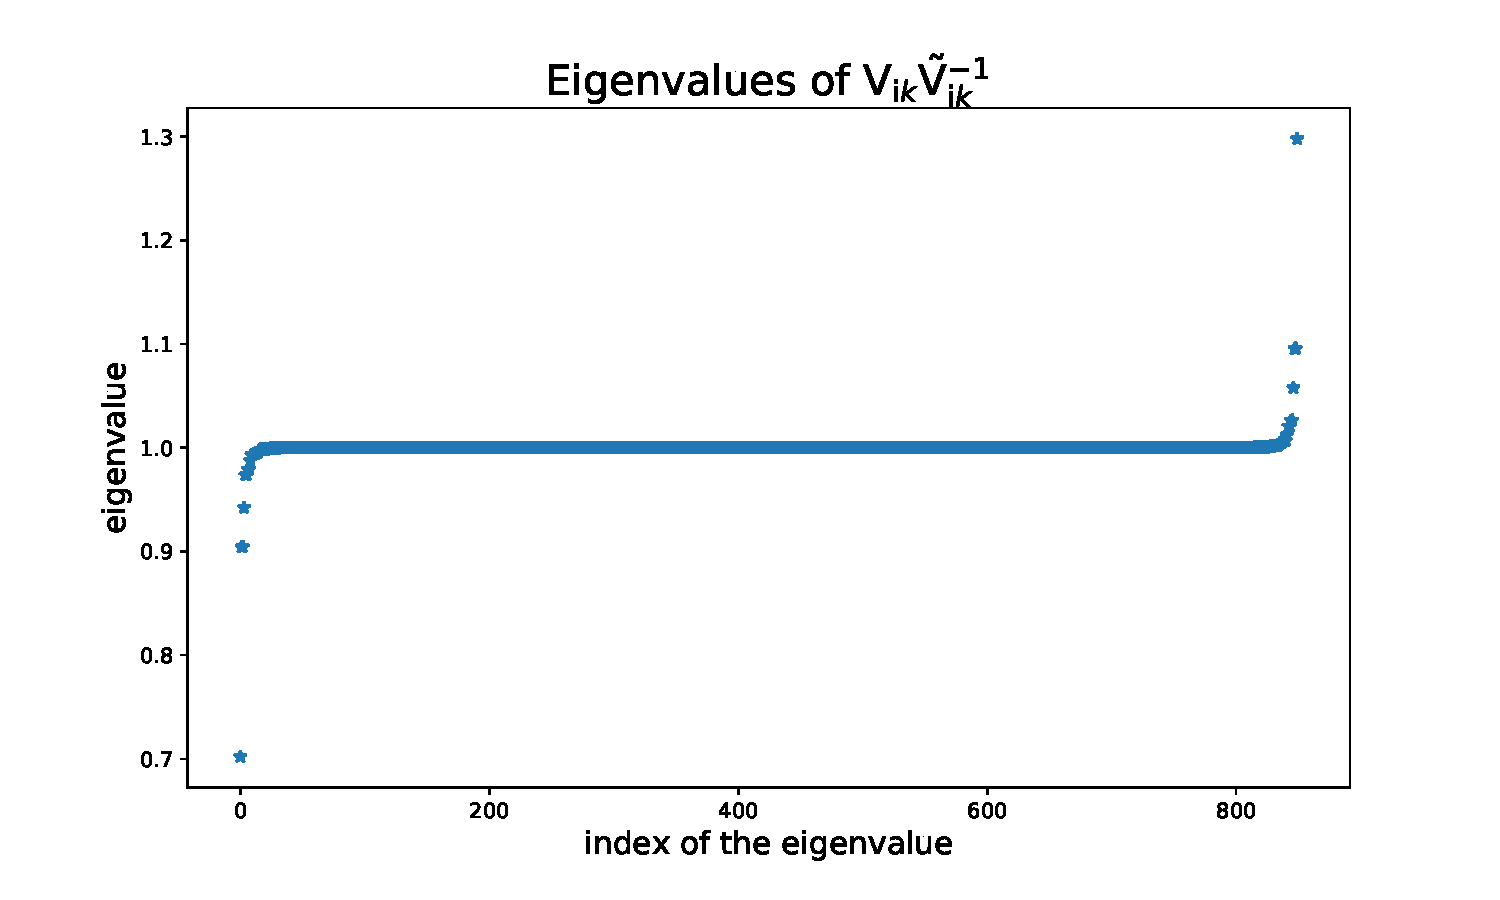
\includegraphics[scale = 0.5]{figures/eigenvalue_of_VVtilde.pdf}
    \caption{The eigenvalues of the matrix $\mathsf{V}_{\mathrm{i}k}\tilde{\mathsf{V}}_{\mathrm{i}k}^{-1}$ when $\mathrm{i}k = 0.8\mathrm{i}$.}
    \label{eigenvalues of VVtilde}
\end{figure}

Consider the eigenvalue problem: 
\begin{align} \label{EP}
    \mathsf{V}_{\mathrm{i}k}\tilde{\mathsf{V}}_{\mathrm{i}k}^{-1}\boldsymbol{x} = \lambda\boldsymbol{x},
\end{align}
where $\lambda$ is the eigenvalue and $\boldsymbol{x}$ is the corresponding eigenvalue. This eigenvalue problem is equivalent to the generalized eigenvalue problem:
\begin{align}\label{GEP}
    \mathsf{V}_{\mathrm{i}k}\tilde{\boldsymbol{x}} = \lambda \tilde{\mathsf{V}}_{\mathrm{i}k}\tilde{\boldsymbol{x}}.
\end{align}
Thus, we can focus on solving the problem \eqref{GEP} instead of \eqref{EP} to avoid computing the matrix inversion. By \cite{golub2002inverse}, the authors 
proposed an inverse free Krylov subspace method for finding the eigenvalues of the symmetric definite generalized eigenvalue problem and the following 
algorithm summarizes this method.

\begin{algorithm}[H]
    \SetAlgoLined
    Input: $m\geq 1$, an initial approximation $\boldsymbol{x}_{0}$ with $||\boldsymbol{x}_{0}|| = 1$; $\rho_{0} = \rho(\boldsymbol{x}_{0}) = \frac{\boldsymbol{x}_{0}^{T}A\boldsymbol{x}_{0}}{\boldsymbol{x}_{0}^{T}B\boldsymbol{x}_{0}}$\\
    Output: The smallest eigenvalue of $A\boldsymbol{x} = \lambda B\boldsymbol{x}$\\
    
    For $k = 0,1,2,...$ until convergence,
    \begin{itemize}
        \item Construct a basis $W_{m} = [\boldsymbol{w}_{0}, \boldsymbol{w}_{1}, \cdots, \boldsymbol{w}_{m}]$ for $K_{m} = \text{span}\{\boldsymbol{x}_{k}, (A - \rho_{k}B)\boldsymbol{x}_{k}, \cdots, (A - \rho_{k}B)^{m}\boldsymbol{x}_{k}\}$
        \item Form $A_{m} = W_{m}^{T}(A - \rho_{k}B)W_{m}$ and $B_{m} = W_{m}^{T}BW_{m}$
        \item Find the smallest eigenpair ($\mu_{1}, \boldsymbol{\nu}_{1}$) for ($A_{m}, B_{m}$)
        \item $\rho_{k+1} = \rho_{k} + \mu_{1}$ and $x_{k+1} = V_{m}\boldsymbol{\nu}_{1}$
    \end{itemize}
    End
     \caption{Inverse free Krylov subspace method for the generalized eigenvalue problem $A\boldsymbol{x} = \lambda B\boldsymbol{x}$}
    \end{algorithm}
    Here, $K_{m}$ is the Krylov subspace with dimension $m$ and $W_{m}$ is the basis of it, which can be obtained through the Arnoldi iteration. 
    
The above algorithm can make us approximate all the eigenvalues of $(A,B)$.

\subsection{Inverse-free method for computing the extreme eigenvalues}
{\color{blue}Show the eigenvalues of the matrix $MM_{\infty}^{-1}$ and introduce the inverse-free method of solving generalized eigenvalue problem 
$Mx = \lambda M_{\infty}x$; then use it to compute the extreme eigenvalues so that we do not have to compute the inverse of $M_{\infty}$ and 
all the eigenvalues of this generalized eigenvalue problem.}